\documentclass[12pt]{article}
\usepackage{amsfonts,amsmath,amssymb,amsthm,epsfig,graphicx,float,tabularx}
\usepackage{booktabs}
\usepackage[margin=1in]{geometry}
\usepackage[font=small]{caption}
\usepackage{wrapfig}
\usepackage{multicol}
\usepackage{braket}
\providecommand{\e}[1]{\ensuremath{\times 10^{#1}}}
%This just let you put stuff to the power of 10 in a nice way

\begin{document}

 \title{Final project proposal}
 \author{Jeffrey Vargas \\ Yash Sanjay ShAh}
 \date{\today}
 \maketitle


%======================================================================================
%=-------------------------------------Introduction-----------------------------------=
%======================================================================================


\section{Introduction:}
Analyzing the spectrum of objects is a common practice in many fields of science. As a result, we are interested in a comprehensive understanding behind spectrometers however, sophisticated spectrometers can be expensive. For our project we want to design and construct a spectrometer. We will use a photo-diode to detect light.

\section{Objective: }
In particular the spectrometer we want to construct involves a circuit which uses a photo-diode to detect light and a combination filters and amps to extract spectrum. Once we extract a spectra we want to use that information and drive a series of color diodes to produce a colorful visual effect.\\

\section{Theory}
The photo-diode works similar to the 1N4448 diode we been using in lab. The photo-diode is a PN junction semiconductor which operates in reverse biased condition. As a result the light incident on the glass lens in the PN junction causes electron pairs to form and a current to flow. 

we plan to use the an op-amp to convert the current to a voltage using the following circuit.

\begin{figure}[H]
\centering
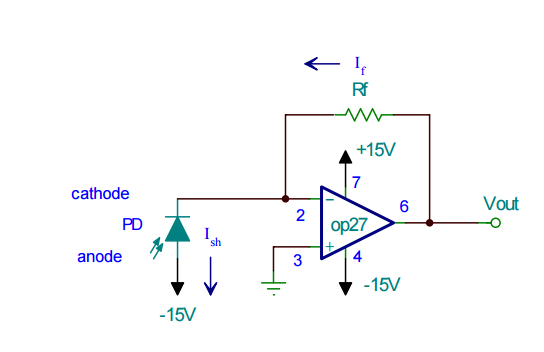
\includegraphics[scale=.5]{image1.png}
\caption{we learn from lab6 that the circuit above is a perfect voltage converter because no current flows through the op-amp}
\end{figure}

since the light in the surrounding environment will create noise in our measurement we will use a high pass filter in order to eliminate low frequency signals.

\begin{figure}[H]
\centering
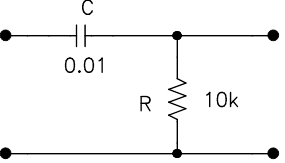
\includegraphics[scale=.5]{highpass.png}
\caption{in lab 1 and 2 we learned that the circuit above is a high pass filter.  }
\end{figure}

Finally we plan to use an amplifier to more precise measurements. the final result would look similar to the circuit below.

\begin{figure}[H]
\centering
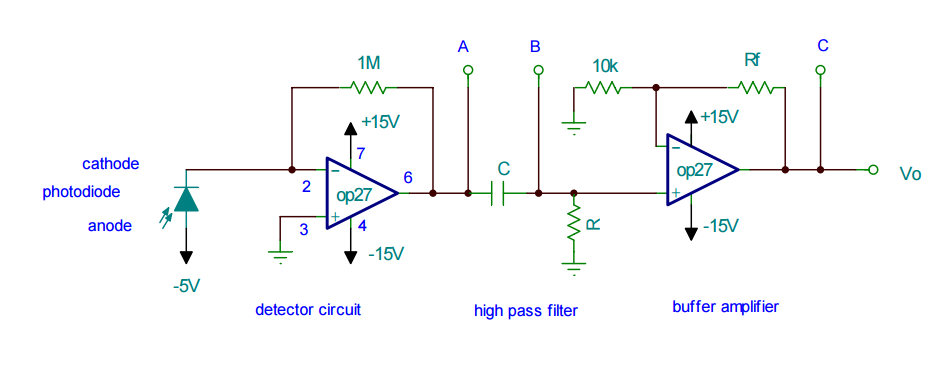
\includegraphics[scale=.5]{spectrometer.png}
\caption{The image was obtained from:\\ https://www.chem.wisc.edu/content/chemistry-524  }
\end{figure}

Next, we plan to extract data using lab view. That informaiton will then be used to drive a series of color LED's. we will then arange them in that shape of a flower. The final result will be a flower mades from color LED's that changes colors depending on the spectrum which is extracted.


\end{document}